\documentclass{article}

\usepackage{graphicx} % Required for inserting images
\usepackage{svg} 
\usepackage{float}
\usepackage[utf8]{inputenc}
\usepackage[T1]{fontenc}
\usepackage{fancyhdr}
\usepackage{pdfpages}
\usepackage{hyperref}
%\makeindex

\title{Rapport í Linux Skipanir}
\author{Salomon Vágadal Joensen, 2022.210\\Jákup Paulason Olsen, 2020.006\\Helena Hentze, 2022.197}
\date{1. Marts 2024}

\begin{document}
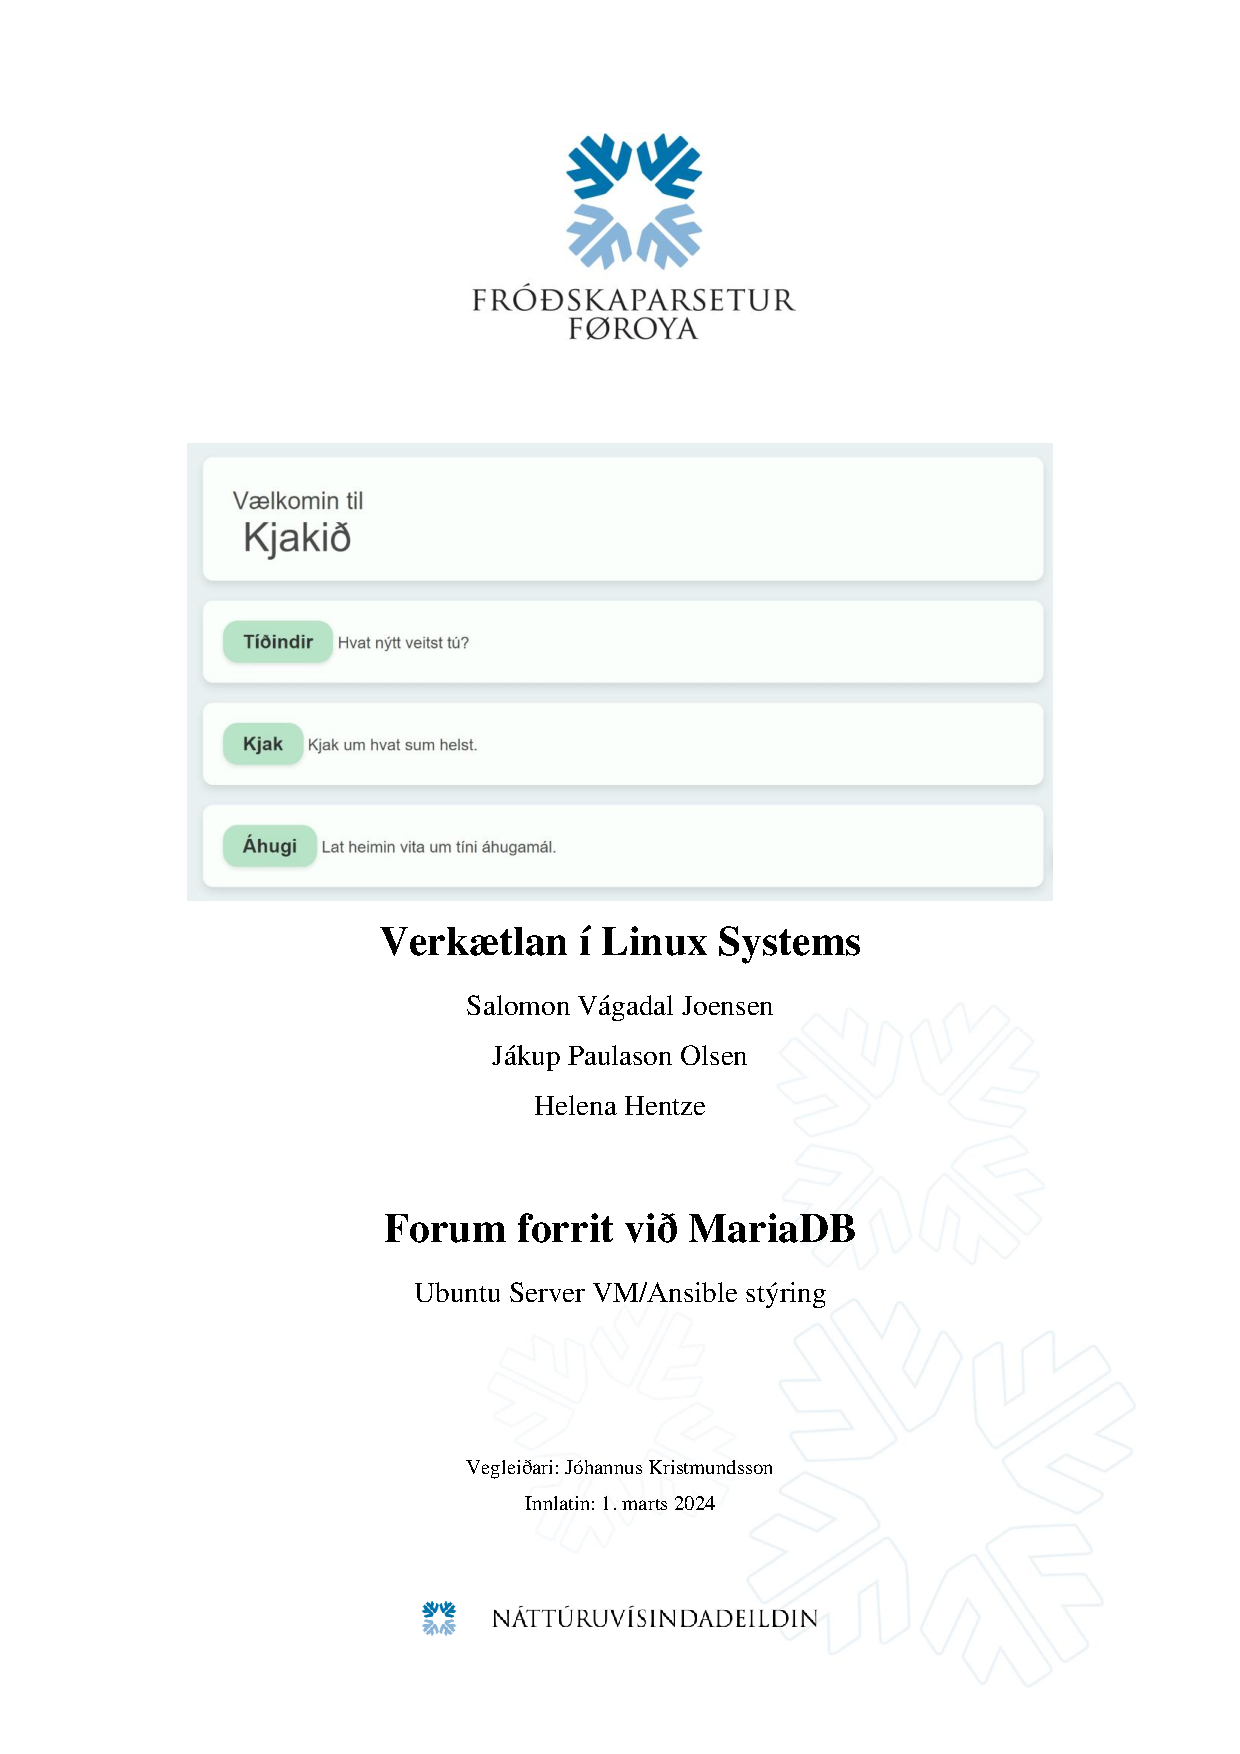
\includepdf[pages=-]{Rapport_frontpage_kjakid.pdf}
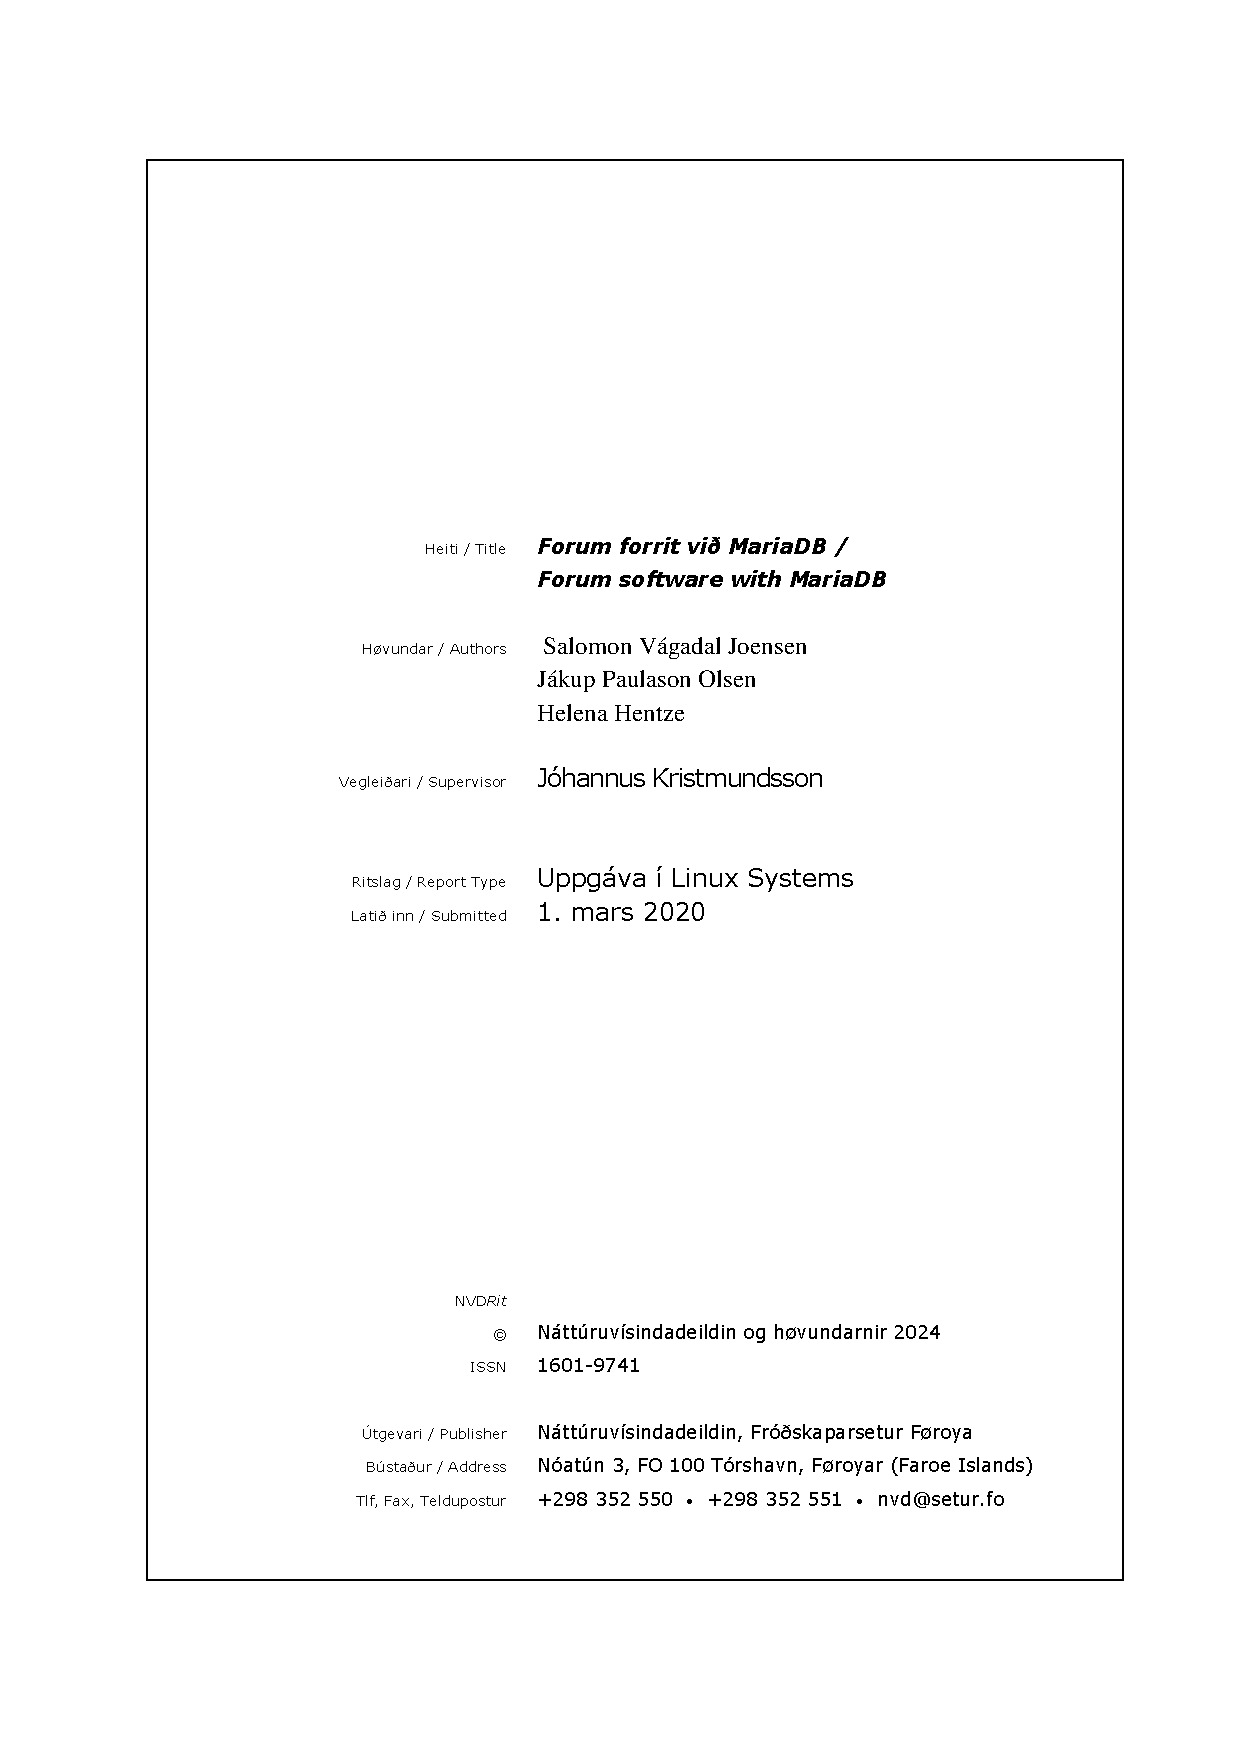
\includepdf[pages=-]{titlepage_kjakid.pdf}
%\maketitle
\tableofcontents
\newpage

\section{Samandrátt (Abstract)}
\par Í hesum rapporti stendur hvussu vit gjørdu eina kjak heimasíðu, hvat fyri tólmenni
(harímillum Ansible, Apache2, MariaDB og PHP) vit brúktu og hvussu arkitektururin var uppbygdur
til at fremja hetta í verki. Eisini verður hugdi at hvussu front-síðan av heimasíðuni verður tillagur, 
so at tað er lætt atkomiligt og gevur brúkarinum yvirlit av heimasíðuni.
til at fremja hetta í verki. Eisini verður hugdi at hvussu front-síðan av heimasíðuni verður tillagur, 
so at tað er lætt atkomiligt og gevur brúkarinum yvirlit av heimasíðuni.

\section{Trupulleika-orðing}
\par Hvussu ger man eina kjak heimasíðu sum fólk kunnu vitja og stovna tráðir og leggja innlegg í? 
Og møguliga eisini hava møguleika at deila media har? 
\begin{itemize}
    \item Man má gera sær greitt at har má vera ein heimasíða, sum fólk vitja.
\end{itemize}

\section{Mál}

\begin{itemize}
    \item Tað má vera lætt at vita hvar man er og hvussu man kemur fram til brúkarin vil vera.
    \item Á hesari heimasíðuni skal brúkarin kunna síggja kjaksíður.
    \item Tað má vera lætt at vita hvar man er og hvussu man kemur fram til brúkarin vil vera.
    \begin{itemize}
        \item Fáa yvirlit av kjak undirsíðunum.
        \item Fara inn á eina kjak undirsíðu.
        \item Síggja tráðir og kunna stovna tráðir.
        \item Kunna fara inn á einkultar tráðir og svara í einum tráði og viðmerkja navn, tekstsvar og um tey vilja leggja mynd avtrat. 
    \end{itemize}
\end{itemize} 

\section{Framgangsháttur}
\par Vit byrja við einari stutta analysu hvussu hetta skal fremjast.
\begin{itemize}
    \item Arkitektur bygnaða av probleminum og hvussu tað fer at síggja út.
    \item Gera ein databasa í MariaDB har man kann stovna ein \textit{thread} í 3 ymiskum kjakforum har fólk kunna svara uppá.
    \item Við einum fullfíggjaðum MariaDB datagrunn byggja eina heimasíðu sum virkar sum eitt \textit{interface} millum heimasíðuna og datagrunnin.
    \item \textit{Business logic} millumlið verður brúkt PHP til samskifting millum
            \newline heimasíðuna og MariaDB.
    \item Millumliðið fer at avgera hvussu úrslit frá datagrunninum verður víst.    
\end{itemize}

\begin{itemize}
    \item HTML verður gjørt fyri at fáa grund bygnaðin av síðuni.
    \item CSS verður nýtt til at pynta HTML og gera snið
    \item JS leggur síðani funktionlatitet til sum ikki hevur við dátabasan at gera
    \item PHP byggur dynamiskt síðuna við at taka postar, tráðir, svør úr dátabasanum
og leggur teir í HTML á síðuni.
\end{itemize}


\section{Design}
\begin{figure}[H]
    \centering
    \includesvg[width=1\textwidth]{html-cs-db.svg} 
    \caption{Samskifti millum heimasíðu og dátagrunnin.}
    \label{fig:html-cs-db.svg}
\end{figure}

\par Ein Ubuntu Server við einari lokalari heimasíðu og brúkt ein MariaDB dátagrunn
at goyma tráðirnir og postar í.
PhpMyAdmin verður brúkt til at síggja dátagrunnin og tað er installera á sjálva servaran,
men er ikki partur av Ansible playbook, tí tað er ikki neyðugt fyri at fáa kjak heimasíðuna
at virka.
\par HTML verður brúkt til at leggja grund til útsjóndina, og so at PHP og JS kunnu peika
til ávis støð tá heimasíðan verður bygt. CSS verður nýtt til at pynta á HTML, fyri at fáa eina
pena og lesiliga heimasíðu. JS verður nýtt fyri at fáa funktionalitet sum at goyma og víðka
tráðir, minka og forstørra myndir. PHP verður brúkt til at dynamiskt byggja lutir av
heimasíðuni, sum t.d. postar, svør og tráðir.

\section{Lýsing av Loysn}

\subsection{Web Uppseting}
\par Lendingar síðan gevur yvirlit av teimum kjakforum sum eru, og leinkir til tey. Brúkarin
velur tað forum teimum ynskir, og verður síðani koyrdur har til. Á kjakforum kunnu tey
hyggja gjøgnum postar, síggja svør og fara ígjøgnum tráðir, samt sum at leggja egnir postir
út ella leggja svar til aðrar postir og onnur svør. Fyri at síggja øll svør má brúkarin fara inn
á postin, og um hann ynskir at síggja tráðir undir svørum til postin trýstir hann á "vís tráð".
Litir eru valdir fyri at geva brúkarinum eina róliga kenslu, og grønt er ofta sett í samband
við ró. Stórar yvirskriftir og stórir knappar eru valdir fyri at vera lættir at lesa. 

%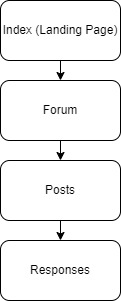
\includegraphics[width=1\includegraphicswidth]{Structure.jpg} 

\begin{figure}[H]
    \centering
    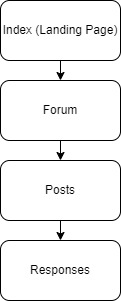
\includegraphics[width=3cm]{Structure.jpg} 
    \caption{Hvussu uppsetingin av forum er.} 
  \end{figure}

\subsection{Databasa Uppseting}

\begin{figure}[H]
    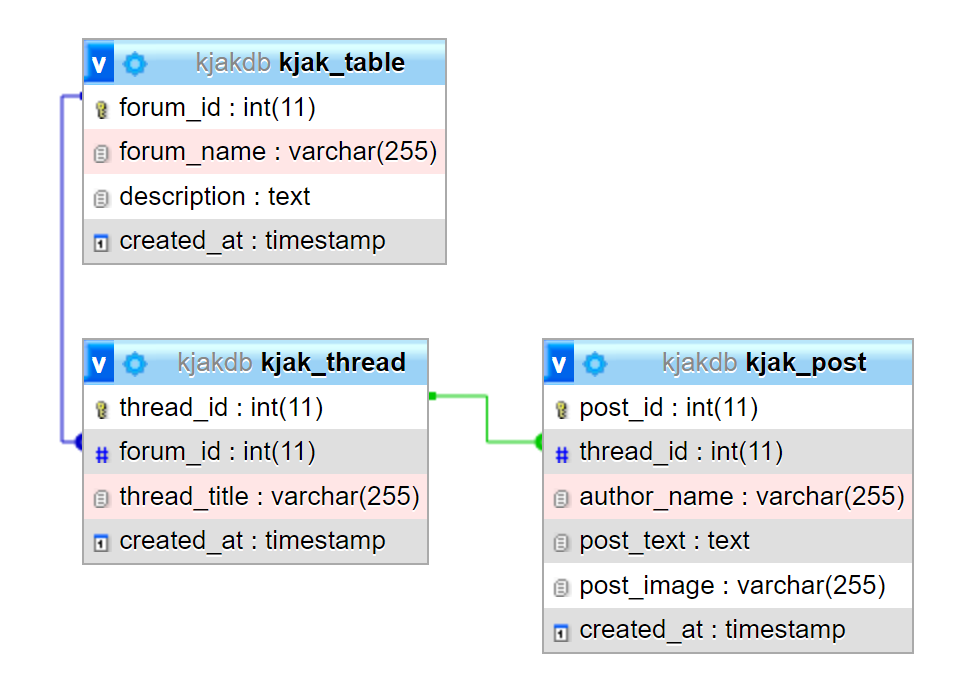
\includegraphics[width=\linewidth]{kjakdb_table_relations.png}
    \caption{Databasa relatiónirnar fyri \textit{kjakdb}}
    \label{fig:kjakdb_table_relations}
\end{figure}

\par Databasa relatiónirnar vísa hvussu
tær 3 tabelirnar eru relatarar. \textbf{kjak\_table} er høvuðs tabellin og hevur
\textit{Primary Key} \underline{forum\_id} til \textit{Foreign Key} til \textbf{kjak\_thread},
og \textbf{kjak\_thread} hevur \textit{Primary Key} \underline{thread\_id} til \textit{Foreign Key}
til \textbf{kjak\_post}.

\subsection{Heimasíðan}
\par Heimasíðan er bert 4 síður við embeddaða PHP kodu til at vísa dáta frá \textit{kjakdb}
dátagrunnins 3 tabellir. Annars er ein CSS fíl \textit{style.css} fyri uppseting
og ein \textit{conn.php} við
íbinding upplýsingarnar til dátagrunnin. Eisini er ein JS fíl \textit{script.js} fyri summar funktónir.
Tær 4 síðurnar eru:
\begin{itemize}
    \item \textit{index.php} \- Heimasíðan sum vísur forumini.
    \item \textit{view\_forum.php} \- Undirsíðan fyri at vísa tráðir fyri eitt forum.
    \item \textit{view\_thread.php} \- Undirsíðan fyri at vísa ein á tráð og allar svør í tí
            tráðinum.
    \item \textit{create\_thread.php} \- Fyri at stovna ein nýggjan tráð.
\end{itemize}

\subsection{Ansible}
\par Hesar 6 fílar (og eisini 7nda \textit{favicon.ico} fílin) verða stovnaðir
av at koyra kommandoina á einari VM við \textit{Ansible}:
\newline
\newline
\fbox{\par \textbf{ansible-pull -U https://github.com/salomonvjoensen/linuxskipanir.git}}
\newline
\par Tað ekskeverarar eina \textit{Ansible} Playbook \textbf{local.yml} á hasum
repository sum ger her hesu trin idempotentli (t.v.s. kann vera endurtikið uttan at
bróta uppá nakað ella gera óneyðug kopiir):
\begin{itemize}
    \item Installerar Apache2, startar Apache2.
    \item Ger eina \textit{uploads} mappu í \textit{/var/www/html/uploads}
    \item Tær 7 fílir kopieraðar yvir til \textit{html} mappuna.
    \item \textbf{MariaDB} tænasta verður stovna og byrja.
    \item \textbf{Pip} og \textbf{PyMySQL} verða installera.
    \item Stovna \textit{kjakdb} dátagrunnin.
    \item Stovna \textit{kjak\_user} brúkaran fyri dátagrunnin.
    \item Koyra SQL script á dátagrunnin fyri at gera tær neyðugu tabellirnar.
    \item Til seinast koyra eitt \textit{bash} script til at dagføra dátagrunnin.
\end{itemize}

 Aftaná kann man opna \underline{localhost} í ein kagara og Kjak heimasíðan er uppi
 og koyrir.

 \par Seinni kann man tillaga ting, so sum brúkarnar \textit{kjak\_user} og \textit{anon}
í \textbf{MariaDB} og dagføra tilsvarandi \textit{conn.php} fílina til teir brúkarnar.


\section{Perspektivisering}
\par Heimasíðan hevur tað mest einklu treytirnar fyri at vera hugsa sum ein kjak-heimasíða,
Síggja nøkur forum, tráðir, stovna tráðir, svara á tráðum og leggja myndir út saman við svør.
\par Tað er ein einkul kjak heimasíða, sum kundi verið nógv útbygt, mest sannlíknandi
kundi verið at vitjandi kundu stovna brúkarar (um tey vildu), so tey sjálvu kundu strika
teirra egnu tráðir og svør. Ting sum at indeksera heimasíðuna, so man kundi leita uppá
dátagrunnin kundi eisini verið implementera.
\par Tað er skjótt at fáa heimasíðuna upp at koyra bara við einari einklari bash kommandoina,
givið man hevur \textbf{Ansible} á einum
Linux líknandi umhvørvi (vit brúktu Ubuntu Server VM), og tað vísur eisini styrkina í \textbf{Ansible}.
\par Vit hugsaðu um at brúka \textbf{Ansible Playbook}, so man kundi havt forriti koyrt á 
fleiri umhvørvum men hvat er meiningin at hava fraktuera kjak á nógvum støðum, tá man kann hava
eitt samla stað at kjakast í?

\section{Niðurstøða}
\par Okkara arbeiði og skeið gav okkum innlit hvussu man brúkar Linux umhvørvi og hvussu tað
er at arbeiða næstan bara í einum terminal uppseting. Nógvar kommandoir skuldi man læra, og
brýtir nógv frá tí vanda GUI umhvørvi man kennur mest frá Windows, men um man dugir kann man
automatisera øgiliga nógv og næstan hálv-forrita redigering av fílum, her hugsi eg um \textit{vim}
editorin.
\par Kjak heimasíðan er einkul, men tøknin aftanfyri er sørmi ikki. Man kundi sett upp heimasíðuna
uttan at hava \textbf{Ansible}, men tað hevði kravt nógv manuelt arbeiði hvørja ferð man skuldi
sett upp eitt nýtt kjak heimasíðu umhvørvi aðra-staðnis.

\section{Appendix}

\subsection{Tíðarætlan}
\begin{figure}[H]
    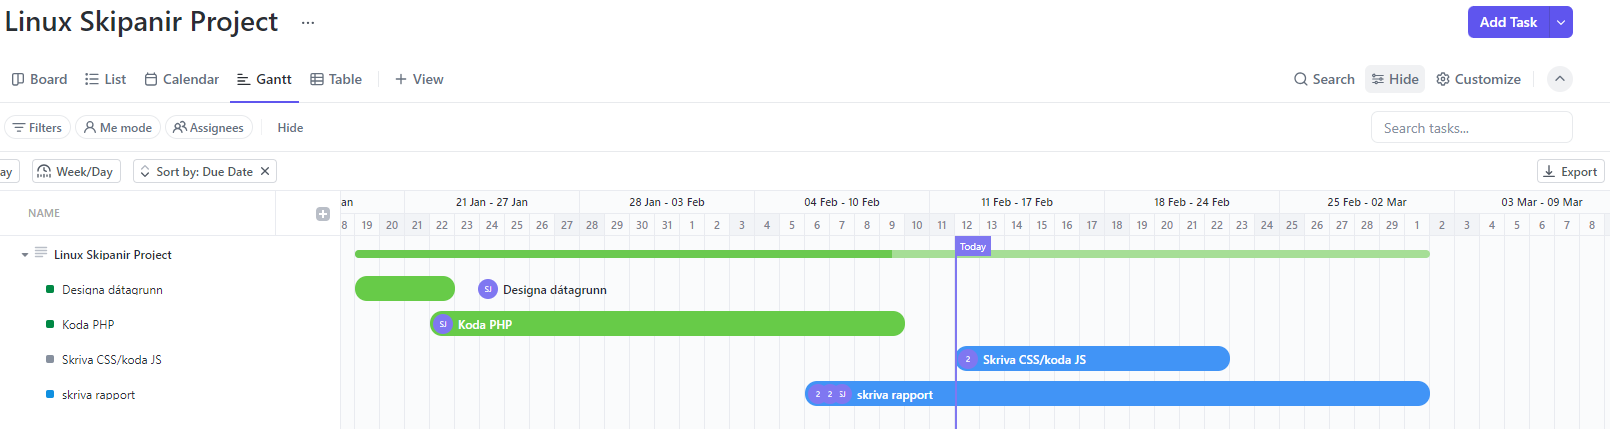
\includegraphics[width=\linewidth]{tíðarætlan.png}
    \caption{Skermmynd tikin av tíðarætlan mánadagin 12. februar 2024}
    \label{fig:tíðarætlan.png}
\end{figure}

\par Fyrst var dátagrunnurin designaður, so bleiv PHP kodan koda til dátagrunnin.
Meðan tað varð arbeiða uppá tað byrjaðu vit so smátt at skriva rapportina og gera tað
seinasta hondverki av HTML, CSS \& JS uppseting av heimasíðuna, bara so hon sær eitt sindur
vøkur út.


\phantomsection
\addcontentsline{toc}{subsection}{kjakdb Schema}
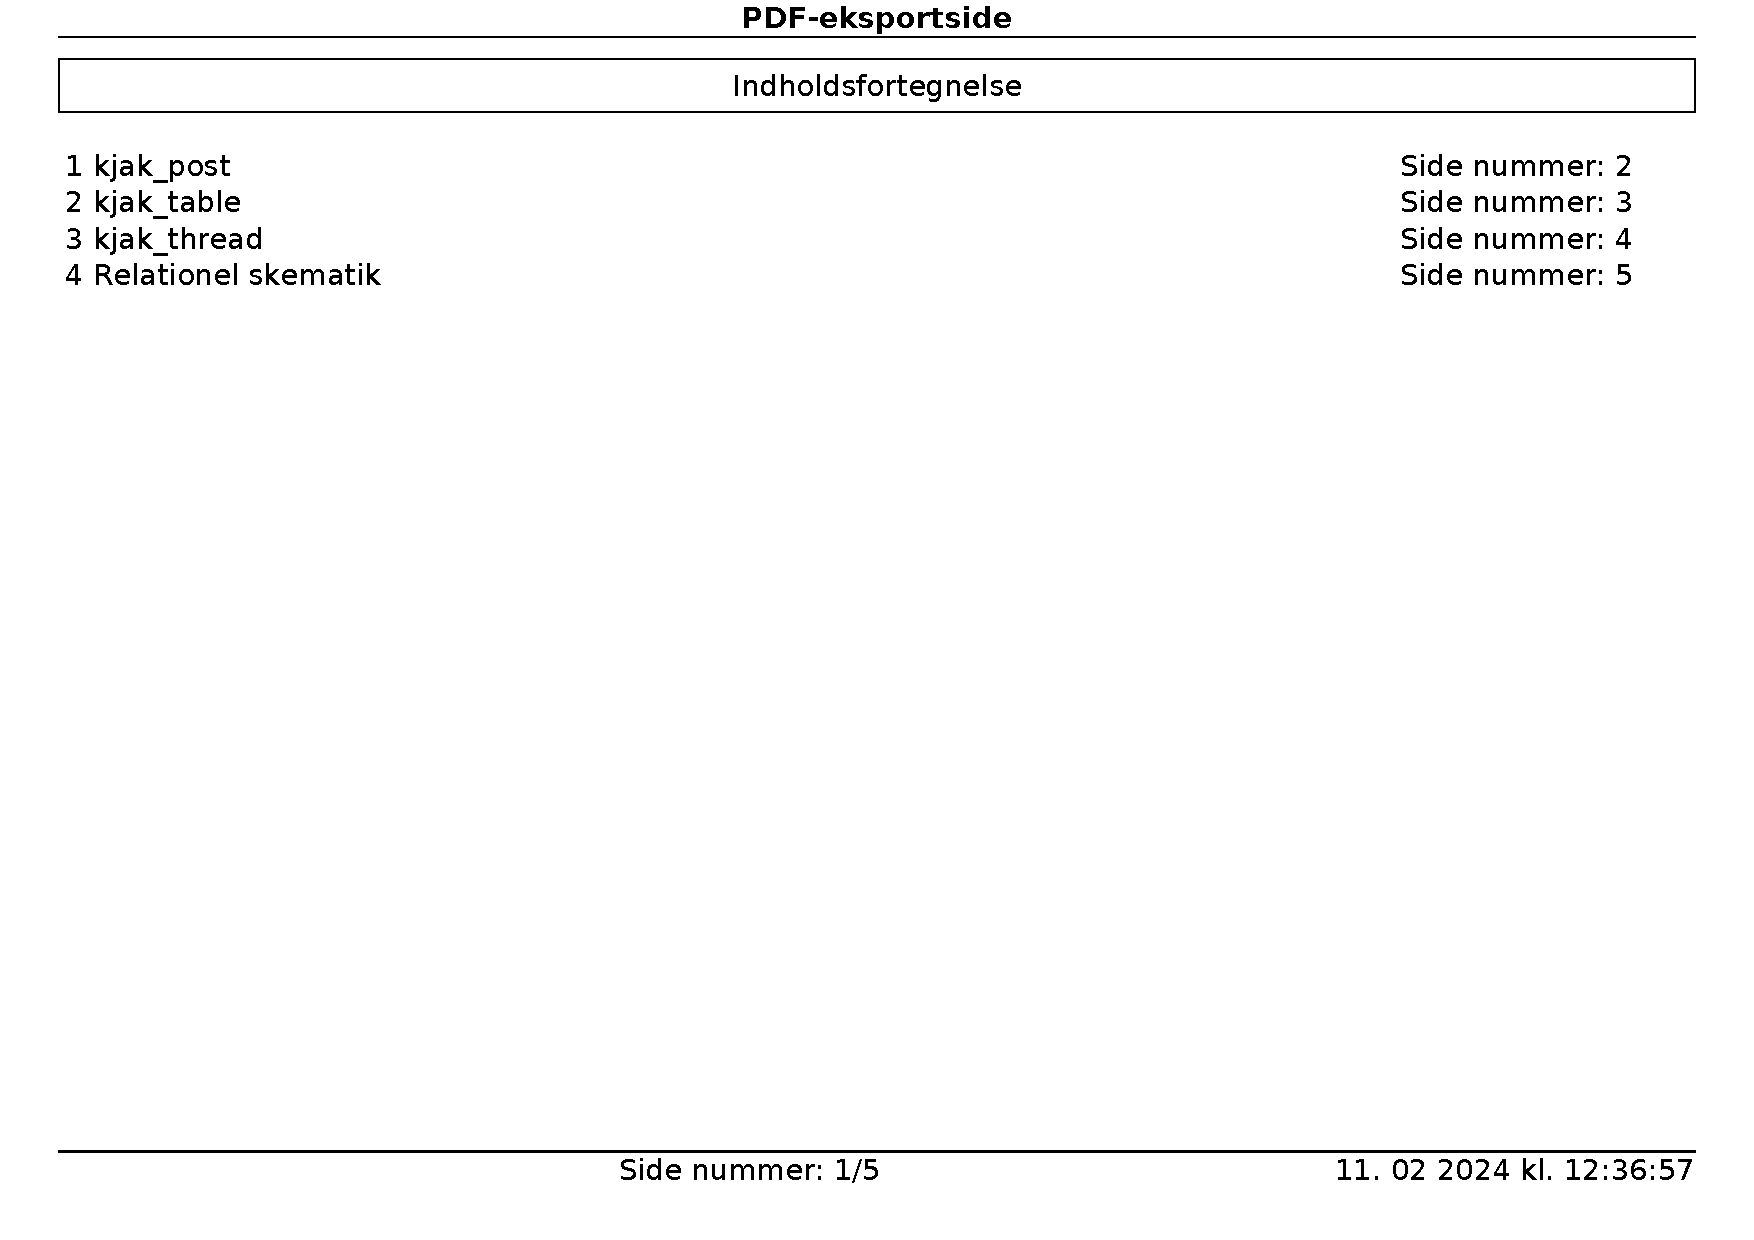
\includepdf[pages=-, pagecommand={\thispagestyle{plain}}]{kjakdb_schema.pdf}

\phantomsection 
\addcontentsline{toc}{subsection}{local.yml}
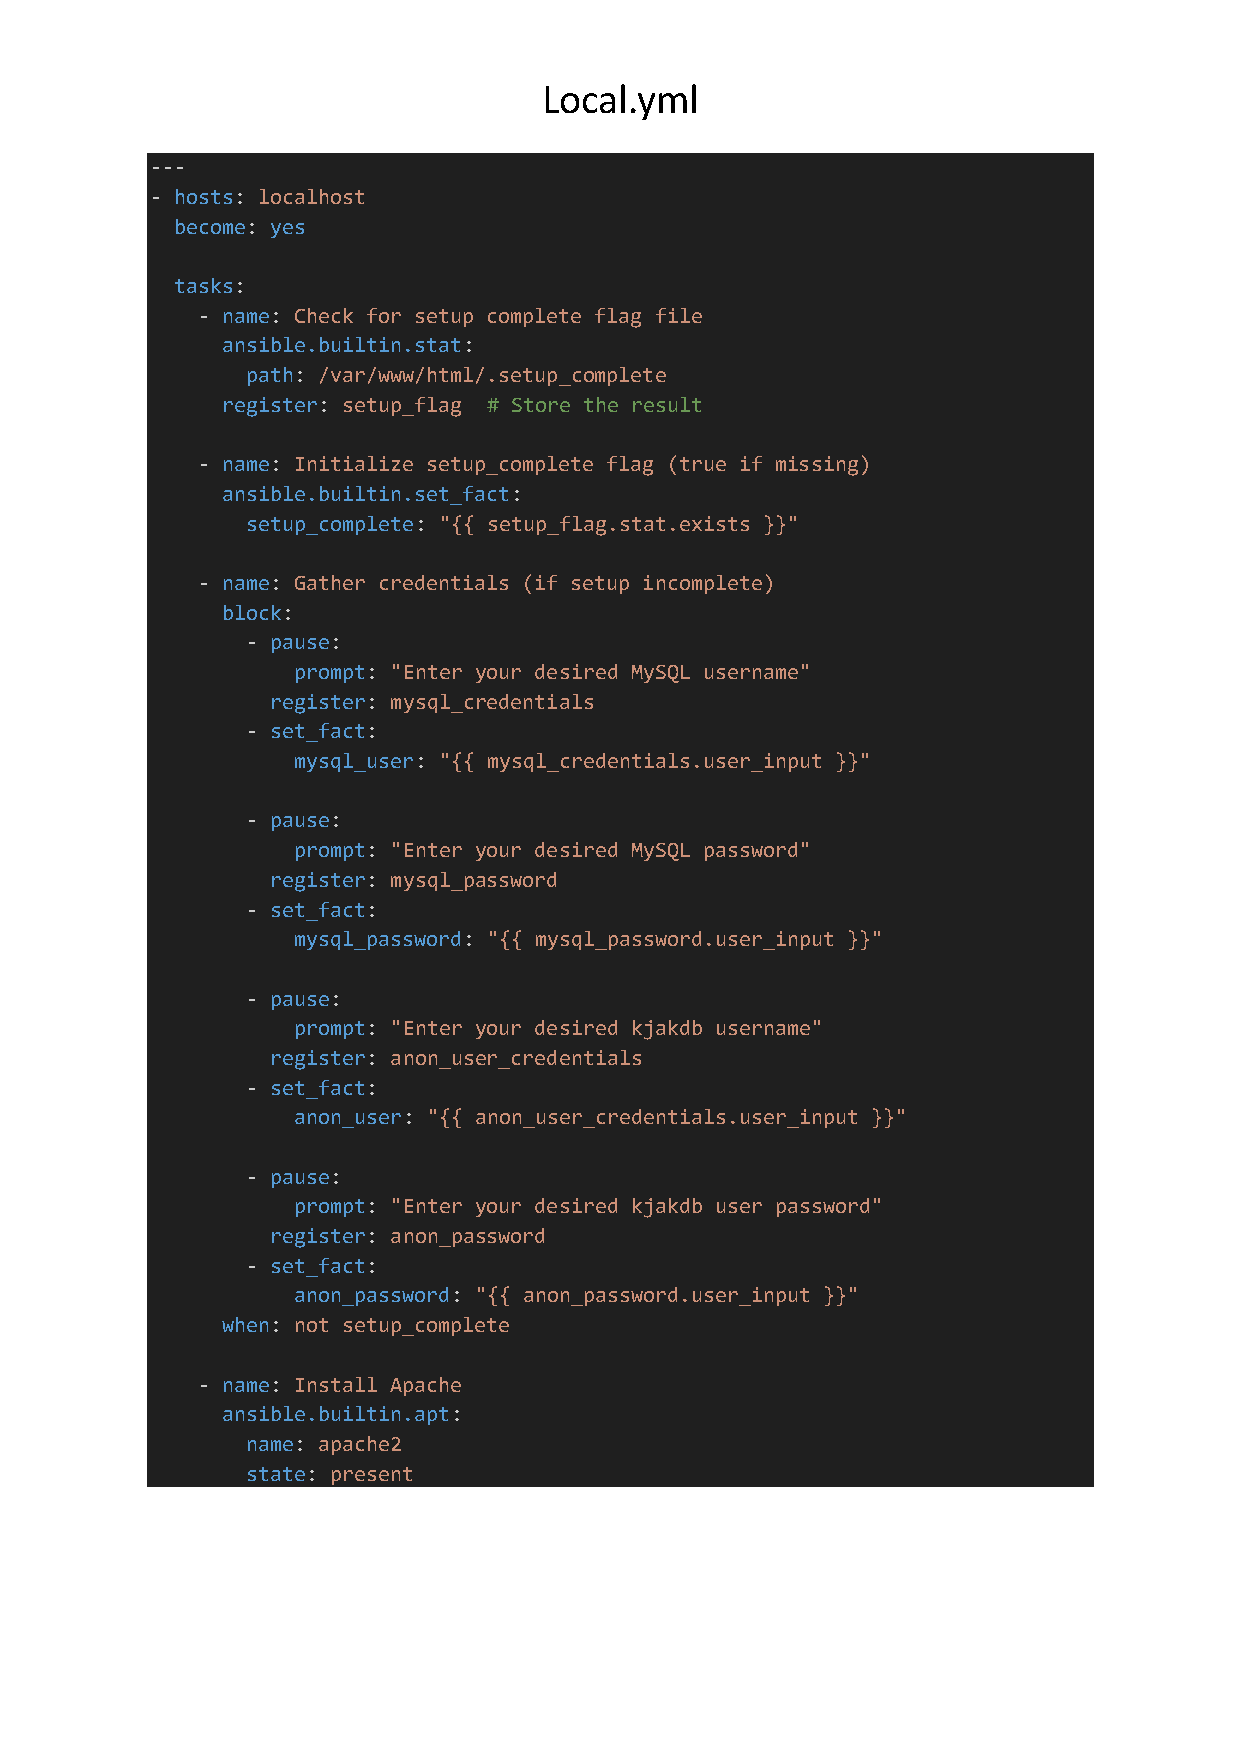
\includepdf[pages=-, pagecommand={\thispagestyle{plain}}]{local.yml.pdf}

\phantomsection 
\addcontentsline{toc}{subsection}{kjakdb.sql}
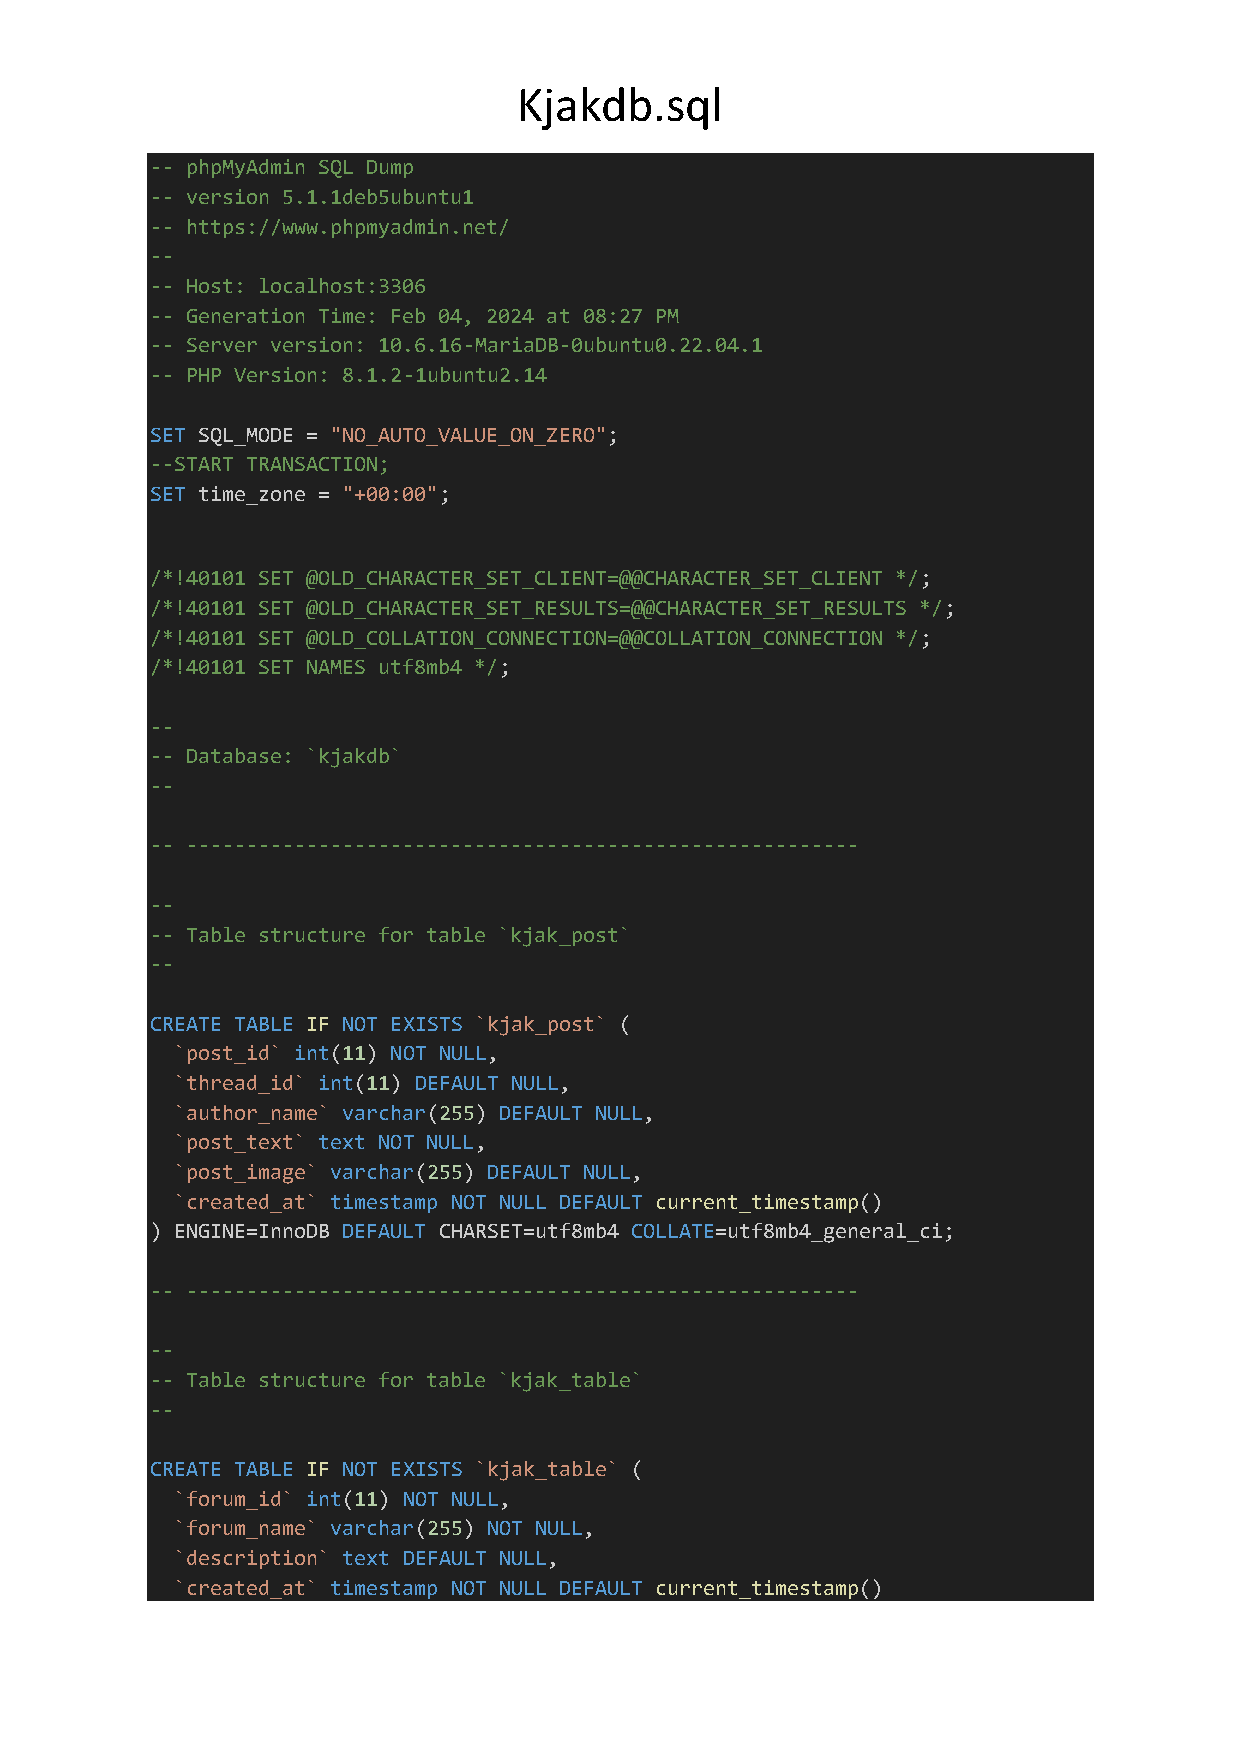
\includepdf[pages=-, pagecommand={\thispagestyle{plain}}]{kjakdb.sql.pdf}

\phantomsection 
\addcontentsline{toc}{subsection}{update\_kjakdb.sh}
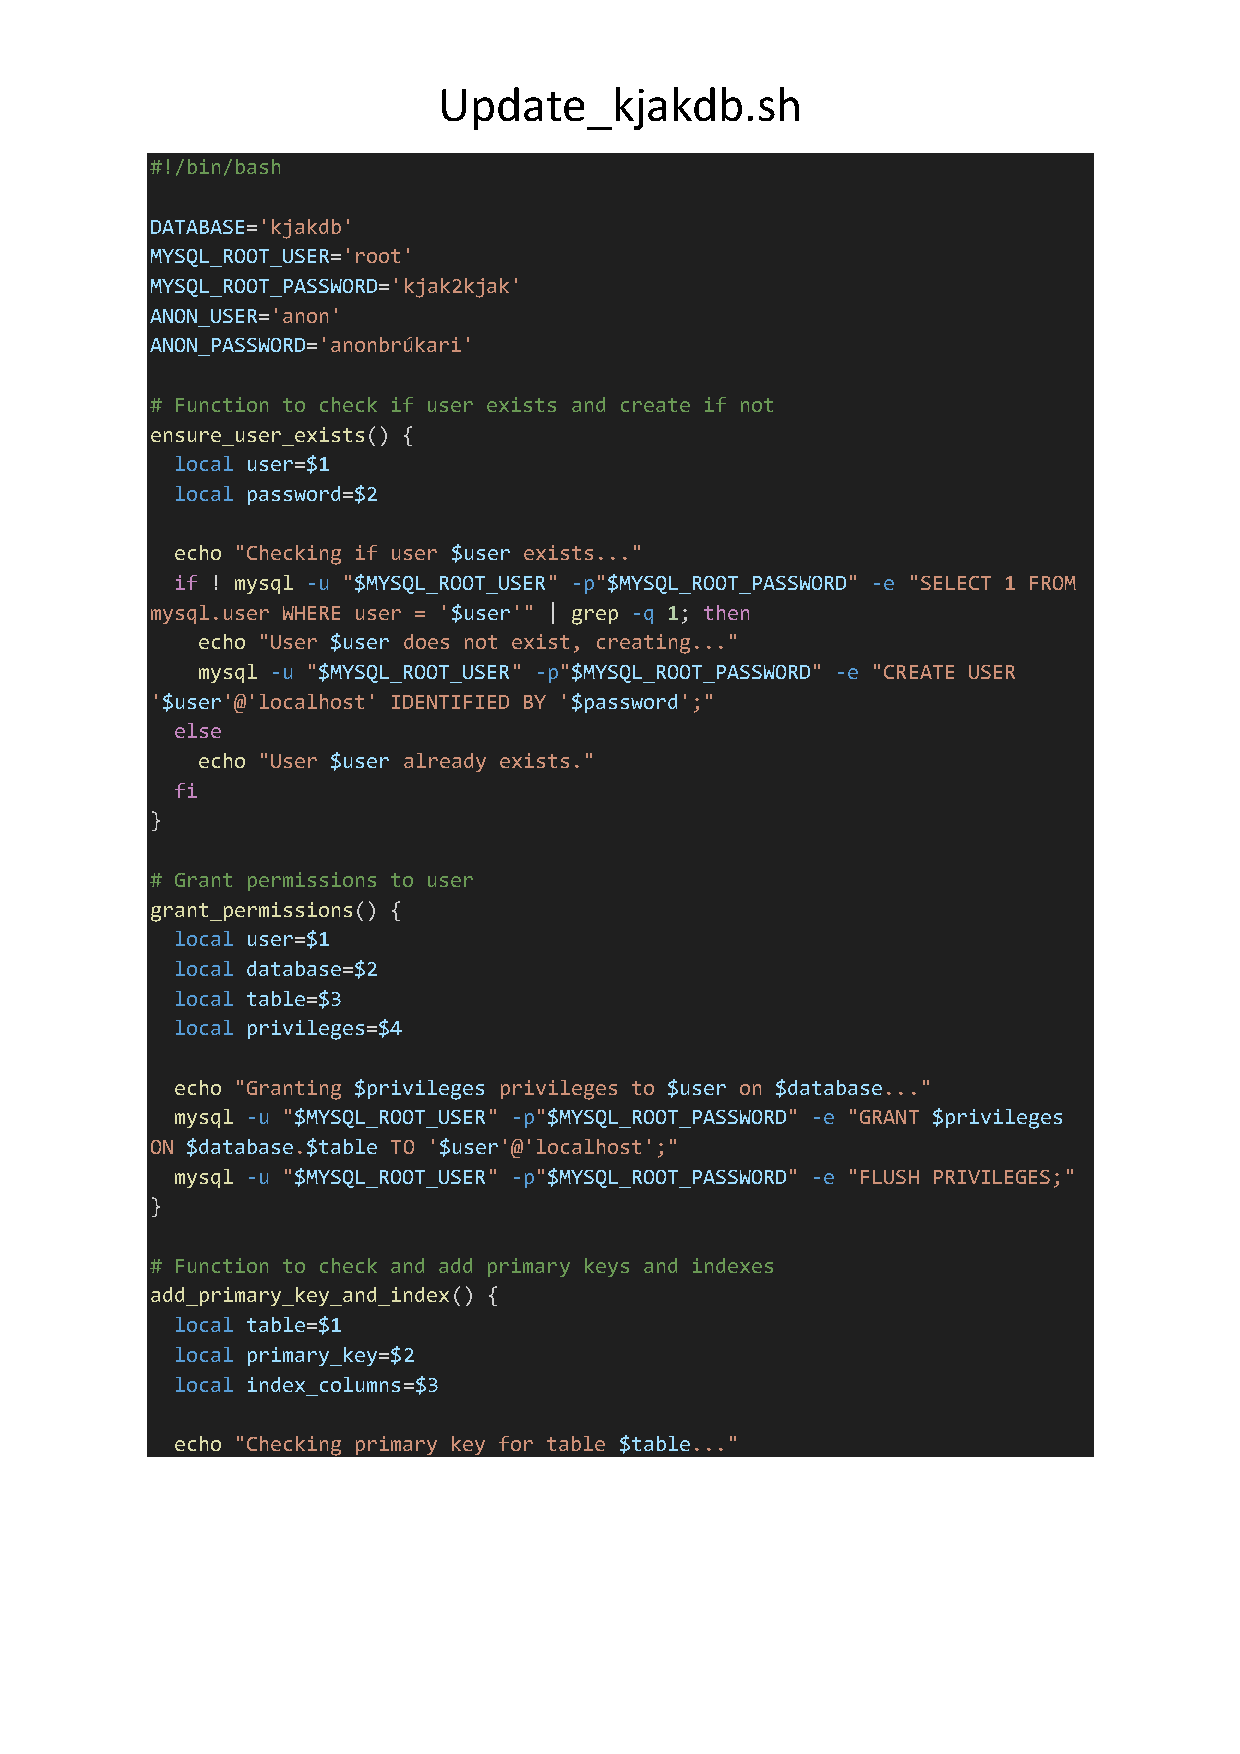
\includepdf[pages=-, pagecommand={\thispagestyle{plain}}]{update_kjakdb.sh.pdf}

\end{document}
